\documentclass[final]{beamer}
\mode<presentation>
{
  \usetheme{I6pd2}
}
\graphicspath{{figures/}} % e.g. where you have your logos

\usepackage{epstopdf}
\usepackage{times}
\usepackage{amsmath,amssymb}
\usepackage[english]{babel}
\usepackage[latin1]{inputenc}
\usepackage{ragged2e} 
\usepackage{multicol}
\usepackage{tabularx}

\usepackage{changepage}

\addtobeamertemplate{block begin}
  {}{\begin{adjustwidth}{1cm}{1cm}}
\addtobeamertemplate{block end}
  {\end{adjustwidth}}

\setbeamertemplate{bibliography item}[text]

\usepackage[orientation=portrait,size=a0,scale=1.4,debug]{beamerposter} 
\title[Fancy Posters]{Manufacturing Cycle with Equiplets}
\author{From User Input to End Product}

\institute{HU University of Applied Sciences Utrecht}
\date{\today}

\newcommand{\columnblock}[2][Title]{
    \begin{block}{\large \vspace{-0.5cm}#1}
    #2
    \end{block}
}

\newcommand{\twocolumnsblock}[3][Title]{
    \columnblock[#1]{
        \begin{multicols}{2}
            #2
            \newpage
            #3
        \end{multicols}
    }
}

\begin{document}
\begin{frame}{}
               % == Introduction == %        
            \columnblock[Introduction]{
            \justifying 
             	In current manufacturing systems, time to market is usually a rather long period. In order to prevent a long time to market, REXOS provides a grid manufacturing system that is highly customizable due to the nature of the production machines (equiplets) that it consists of. All the equiplets in the grid are reconfigurable and thus are able to provide a variety of services resulting in a high mix low volume production grid. This poster shows the lifecycle of a product from input to production within such a grid.
            }
    % == Manufacturing Cycle == %
    \columnblock[Manufacturing Cycle]{
            \justifying 
    \includegraphics[width=.98\linewidth]{ProductCycle}
    }
    
	\begin{columns}[t]
			% ====== START OF COLUMN B ===== % 
    	\begin{column}{0.35\linewidth}    	
            
             % == Finding the Right Equiplets == %
            \columnblock[Finding the Right Equiplets *]{
            \justifying 
            Once the blueprint for a product is known, the product agent will need to know where the product can be produced. The product agent will start by asking each equiplet in the grid whether it is capable of performing the needed steps. The equiplets have capabilities which are based on the modules attached and therefor the services it provides. If an equiplet has the right capability to perform a step, it will inform the product agent providing a duration of how long the steps will take to execute. 
            }
		\end{column}
		
		\begin{column}{.63\textwidth}
			% == Image == %
			\columnblock[Example Translating Steps **]{
            \justifying 
			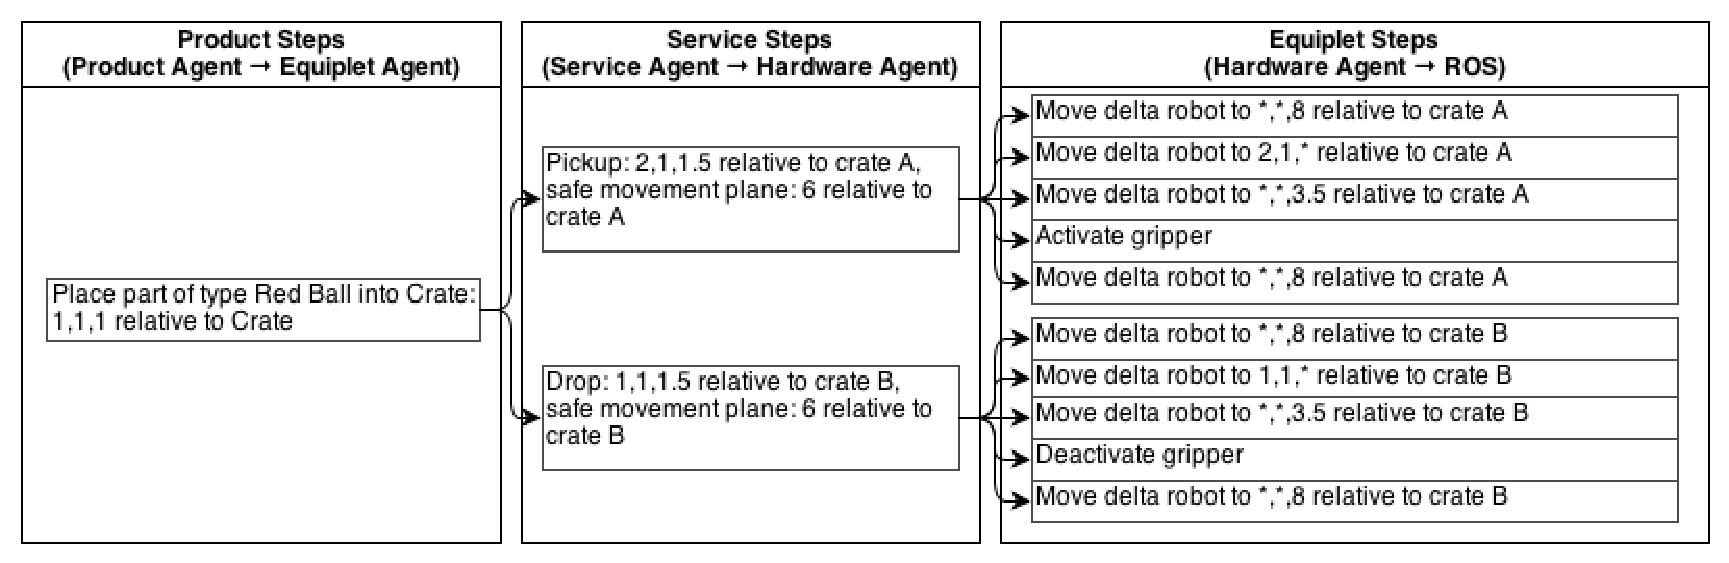
\includegraphics[width=.98\linewidth]{product-abstraction.eps}
			}
    	\end{column}
		% ====== END OF COLUMN A ====== %

	\end{columns}
           
   \columnblock[Product Life after Production]{
    \justifying 
	The resulting product logs can be used in different situations. These product logs can be consulted in order to optimize production. Future services, such as generating schematics for repairing the product, can be developed using these detailed production logs.
}
           
\end{frame}
\end{document}